\documentclass{fizraport}
\authorA{Krzysztof Stasiowski}
\authorB{Joanna Binek}
\usepackage[version=4]{mhchem}
\usepackage{adjustbox}

\team{2}{2a}{1}

\topic{Elektroliza }{35}{
Wyznaczenie stałej Faradaya oraz~równoważnika elektrochemicznego miedzi metodą
elektrolizy.}
\carryOutDate{07.11.2018 r.}
\ftHandInDate{14.11.2018 r.}
\begin{document}
\maketitle

\section{Wstęp teoretyczny}
Charakterystyczną grupę przewodników prądu elektrycznego stanowią elektrolity. Elektrolit powstaje gdy struktura krystaliczna rozpuszczanej substancji, rozpada się~(dysocjuje) na~jony, które następnie poruszają się~bezładnie po~roztworze. Gdy w~elektrolicie zanurzymy elektrody i~podłączymy je~do~źródła stałego prądu,
ruch jonów stanie się~uporządkowany i~zacznie płynąć przez niego prąd -~kationy podążają do~ujemnej katody, a~aniony do~dodatniej anody.
Na~elektrodach jony zostają zobojętnione i~stają się~zwykłymi atomami lub~zgrupowaniami atomów. Przepływowi prądu towarzyszy więc wydzielanie się~substancji na~elektrodach.Proces ten~nazywamy elektrolizą. 

Aby jon mógł zostać zobojętniony na~elektrodzie, musi przepłynąć ładunek równy $w\cdot e$, gdzie~$e$~-~ładunek elementarny elektronu, a~$w$~-~wartościowość jonu.
Liczbę atomów które wydzieliły się~na~elektrodzie możemy wyznaczyć jako~stosunek całkowitego ładunku ($I \cdot t$) do~ładunku pojedynczego jonu ($we$)
\begin{equation}
N=\frac{It}{we}
\end{equation}
Masę osadzonych atomów można obliczyć mnożąc ich~ilość przez masę jednego atomu. Masę pojedynczego atomu można wyznaczyć jako~stosunek masy molowej do~liczby Avogadra, stąd
\begin{equation}
\label{eq:masa}
m=N\frac{\mu}{N_A}=\frac{\mu}{weN_A}It
\end{equation}

Można zauważyć, że masa wydzielonej substancji jest~proporcjonalna do~natężenia prądu $I$,\\ czasu~przepływu prądu $t$~oraz~współczynnika 
\begin{equation}
\label{eq:k}
k=\frac{\mu}{weN_A}
\end{equation}
oznaczanego $k$~i~zwanego elektrochemicznym równoważnikiem substancji.

Iloczyn $eN_A$ wyraża ładunek potrzebny do~wydzielenie jednego gramorównoważnika chemicznego substancji. Oznacza się~go~zwykle jako~$F$~i~nazywa stałą Faradaya.
Ze~wzoru (\ref{eq:k}) wynika jego~zależność od~$k$:
\begin{equation}
F=\frac{\mu}{wk}
\end{equation}

\newpage %można pomyślec nad mniejszym marnotrawieniem papieru w~celu dołączenia naszych ręcznych zagadneń kontrolncyh
\addtocounter{page}{2}%żeby nasze kartki były zawarte w~numeracji



\section{Opis doświadczenia}
\subsection{Układ pomiarowy}
\begin{enumerate}
    \item Naczynie do~elektrolizy siarczanu miedzi \ce{CuSO4}  z~miedzianymi elektrodami w~kształcie równoległych płyt, oddalonych od~siebie o~kilka centymetrów (\figref{fig:schemat}).
    \item Zasilacz napięcia stałego
    \item Amperomierz
    \item Opornica suwakowa
    \item Waga elektroniczna
\end{enumerate}
\begin{figure}[!htb]
\centerline{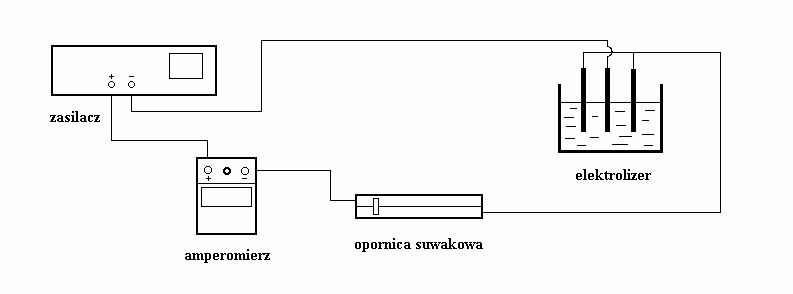
\includegraphics[scale=0.7]{5/schemat-obw.png}}
\caption{Schemat wykorzystanego obwodu elektrycznego}
\label{fig:schemat}
\end{figure}
\subsection{Wykonane czynności}
W~pierwszej kolejności połączaliśmy obwód zgodnie z~podanym schematem. Następnie oczyściliśmy elektrody przy~pomocy papieru ściernego i~wody destylowanej,osuszyliśmy je~i~zważyliśmy.

Po~umocowaniu elektrod na~statywie, zanurzyliśmy je~w~elektrolicie. Prąd płynący przez~roztwór został ustalony na~$0.55A$.

Po~sprawdzeniu obwodu przez prowadzącego zajęcia i~podaniu czasu trwania elektrolizy (25 minut) włączyliśmy zasilacz i~uruchomiliśmy stoper. Przy~pomocy opornicy suwakowej ustaliliśmy zadaną wartość natężenia prądu. 

Po~upływie zadanego czasu elektrolizy wyłączyliśmy zasilacz, wyjęliśmy elektrody z~woltametru i~wymontowaliśmy katodę. Celem usunięcia ewentualnego osadu przepłakaliśmy je~wodą destylowaną,\\ a~następnie wysuszyliśmy przy~użyciu suszarki.

Na~koniec zważyliśmy ponownie katodę i~anody.


\section{Wyniki pomiarów}
\begin{table}[htb]
\centering
\caption{Wyniki pomiarów masy elektrod}
\begin{tabular}{|r|r|r|r|}
\hline
\multicolumn{1}{|l|}{} & \multicolumn{1}{c|}{anody} & \multicolumn{1}{c|}{katoda} \\ \hline
masa przed $[g]$       & 276.653                     & 132.745 \\ \hline
$u(m)~[g]$             & 0.001                       & 0.001  \\\hline          
masa po~$[g]$          & 276.376                     & 133.022 \\ \hline
$u(m)~[g]$             & 0,001                       & 0.001  \\ \hline
$\Delta m~[g]$         & 0.2770                      & 0.2770 \\ \hline
$u(\Delta m)~[g]$      & 0.005                       & 0.005   \\ \hline
\end{tabular}
\end{table}

\begin{itemize}
    \item  Czas trwania elektrolizy: $\SI{25}{\min}=\SI{1500}{\sec}$
    \item  Natężenie prądu $I=\SI{0.55}{\ampere}$
\end{itemize}

\newpage %pomiary
\addtocounter{page}{1}%żeby nasze kartki były zawarte w~numeracji


\section{Opracowanie wyników}
\begin{itemize}
\item Przyrost masy na~katodzie: $0.2770~g$
\item Ubytek masy na~anodach: $0.2770~g$
\item Niepewność: $u(I) = \frac{klasa  \cdot  zakres}{100} = \frac{0,5 \cdot 0,75}{100}=\SI{3,75}{\milli\ampere}$
\item Niepewność: $u(T) = \SI{2}{\sec}$~-~z~powodu niewielkiej wartości niepewności pomiaru czasu \\-~$0.13\%$~-~uznajemy ją~za~pomijalnie~małą.
\end{itemize}

\subsection{Obliczenie współczynnika elektrochemicznego miedzi $k$}
$$k=\frac{m}{It}=\frac{0.2770}{0.55 \cdot 1500}= \SI{0.336}{\milli\gram\per\ampere\per\second}$$

\begin{align*}
	\frac{u(k)}{k} &= \sqrt{ \left(\frac{u(m)}{m} \right)^2 + \left(\frac{u(I)}{I} \right )^2 } \\
	&= \sqrt{ \left(\frac{0,01}{0.2770} \right)^2 + \left(\frac{0,00375}{0,55} \right )^2 }=0.037
\end{align*}

$$u(k) =  0.037  \cdot  0.336=\SI{0.013}{\milli\gram\per\ampere\per\second}$$

\subsection{Obliczenie stałej Faradaya $F$}

\begin{align*}
    F &= \frac{\mu}{wk} \\&= \frac{63540}{2 \cdot 0.336} = \SI{94600}{\coulomb\per\mol}
\end{align*}

Stała Faradaya jest~wyliczona poprzez podzielenie wartości tablicowej $\mu$ ~-~o~pomijalnie małej niepewności, poprzez $k$~stąd można wyliczyć ją~ze~wzoru:

\begin{align*}
	\frac{u(F)}{F} &= \sqrt{ \left[\frac{u(k)}{k} \right]^2 + \left[\frac{u(\mu)}{\mu} \right ]^2 } 
	=  \sqrt{ \left[\frac{u(k)}{k} \right]^2 } = \frac{u(k)}{k}\\
	u(F) &= F\cdot\frac{u(k)}{k}=  94600.00\cdot0.037 = \SI{3500}{\coulomb\per\mol}
\end{align*}
\subsection{Obliczenie ładunku elementarnego $e$}
Ładunek elementarny możemy obliczyć przekształcając wzór~$F=e \cdot N_A$~do:
$$e=\frac{F}{N_A}$$
$$e=\frac{94600}{6.02 \cdot 10^{23}}=1.5718 \cdot 10^{-19}C$$

$$u(e)=\sqrt{\left(\frac{\delta e}{\delta F} \cdot u(F) \right)^2}=\frac{u(F)}{N_A}=\frac{3500}{6.022 \cdot 10^{23}}= 5.9 \cdot 10^{-21}C$$

\newpage
\section{Podsumowanie}
\begin{table}[!htb]
\centering
\footnotesize
\def\arraystretch{1.7}
\begin{adjustbox}{center}
\begin{tabular}{|l|l|l|l|l|l|c|}
\hline
	& \begin{tabular}{@{}c@{}}Wartości\\obliczone\end{tabular}	& \begin{tabular}{@{}c@{}}Wartości\\tablicowe\end{tabular}
	& Różnica	& \begin{tabular}{@{}c@{}}Niepewność\\standardowa\end{tabular}
	& \begin{tabular}{@{}c@{}}Niepewność\\rozszerzona dla $k=2$\end{tabular} & \begin{tabular}{@{}c@{}}Zgodność z~wartością\\tablicową $|x-x_0|<U(x)$\end{tabular}		\\ \hline
$k~[\frac{mg}{C}]$
& $0.336$
& $0.329$
& $0.007$  
& $0.013$
& $0.026$
& tak~					
\\ \hline
%
$F~[\si{\coulomb\per\mol}]$				
& $94600$				
& $96500$					
& $1900$    
& $3500$			
& $7000$			
& tak~			
\\ \hline
%
$e~[C]$				
& $1.5718 \cdot 10^{-19}$		
& $1.6021 \cdot 10^{-19}$	
& $3.0 \cdot 10^{-21}$	
& $5.9 \cdot 10^{-21}$	
& $11.8 \cdot 10^{-21}$	
& tak~	
\\ \hline
\end{tabular}
\end{adjustbox}
\end{table}
%to do: , podsumowanie
 Wyniku dokładnego przeprowadzenia doświadczenia i~precyzyjnych przyrządów, wyliczone wartości stałej Faradaya, współczynnika elektrochemicznego oraz~ ładunku elementarnego są~w~granicach niepewności rozszerzonej zgodne z~wartościami tablicowymi.
\end{document}
